%---------------------------------------------------------------------------
% System tests.
%
%---------------------------------------------------------------------------


\section{Sytem Tests}
\label{sec:ch7_tests}

\subsection{Test Setup}

In order to evaluate system performance abilities and to find potential bottlenecks, performance tests where performed. Due to lack of resources, test setup where rather simple. For test purposes I have used 2 machines: 
\begin{itemize}
\item {\bf HP nx6110} laptop having Pentium M 1.73 GHz CPU and 1.5GB of RAM, running Ubuntu Linux
\item {\bf Sony Vaio VPCEB2Z1E}, with Pentium i5 M430, running at 2.24GHz with 2 physical cores and two processing pipelines running on each core, additionally having 4GB of RAM. This machine was running under control of Microsoft Windows7.
\end{itemize}
HP nx6110 Laptop with Pentium M 1.73Ghz and 1.5GB of RAM memory as computer running sample application that will be monitored and Sony Vaio VPCEB2Z1E, with Pentium i5 M430, running at 2.24GHz with 2 physical cores and two processing pipe lines running on each core, additionally having 4GB of RAM. Those machines where connected using 100Mb Fast Ethernet switch.

Test scenario was composed of following steps:

\begin{enumerate}
\item Launch Monitoring Hub Application module
\item Launch GUI module
\item On separate machine launch 3 JVM processes that mimic processing workflow
\item Again, on testing machine launch iptraf to have insight to network load
\item Launch 2 JProfiler\footnote{\url{http://www.ej-technologies.com/products/jprofiler/overview.html}} instances, attach them to GUI and Monitoring Hub processes
\item Using GUI module and external Monitoring Hub Application started in previous step, add all 3 JVMs as measured resources
\item Create 20 sample measurements, covering: Memory usage, CPU usage, per process Heap and Non Heap memory usage
\item Create 5 Visualizations, using all types system supports and measurements created in previous step
\item Let the system running to gather performance data having system on severe load
\item Dispose visualizations
\item Dispose measurements
\item Remove resources
\item Leave system running for short period of time, to make sure that CPU and memory usage returns to values from idle state
\end{enumerate}

In designed scenario, I am using external Monitoring Hub Application to verify resources usage of each component separately. Additionally, HP laptop was running test application and Vaio was running monitoring system. I have decided to use those resources in that way, to make sure that system being tested will not reach machine limits to be certain that results aren\rq{}t polluted with edge conditions. Results of tests  can be found in following subsections, separate for each module.

\subsection{Tests Results - GUI module}


\begin{figure}[ht]
  \centering
  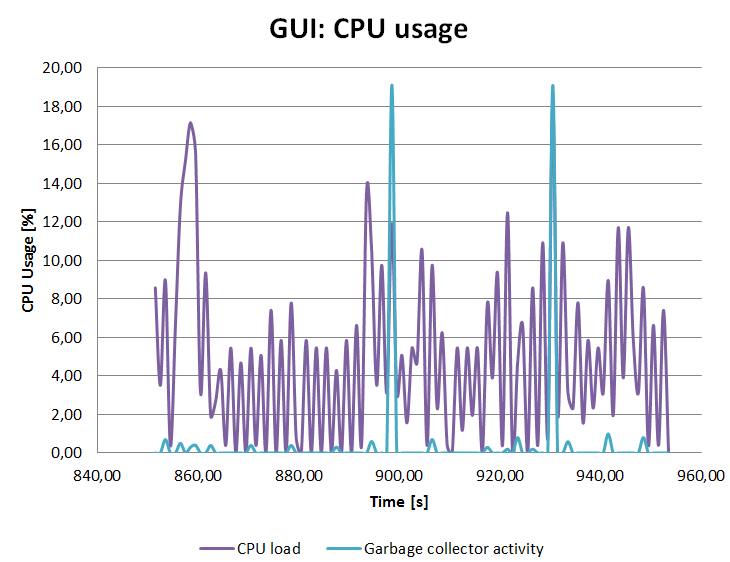
\includegraphics[width=0.6\textwidth]{prof_GUI_CPU}
  \caption{Profiling results of GUI component - CPU usage perspective}
  \label{fig:prof_GUI_CPU}
\end{figure}

Figures~\ref{fig:prof_GUI_CPU}~and~\ref{prof_GUI_MEM}~contains JVM telemetry measurements produced by JProfiler during stage of tests where system where operating under heaviest load (Step~9 from steps list). As can be seen, system never consumed more than 90MB of used memory. The maximum of commit memory slightly exceeded 140MB. On the other hand, the CPU time spent on actual data processing  never reached 18\%, having an average between 2\% and 8\%. What is quite interesting is the Garbage Collection, most of the time CPU time spent on garbage collection was hardly traceable, but there where 2 peaks where GC consumed nearly 20\% of CPU time. 


\begin{figure}[ht]
  \centering
  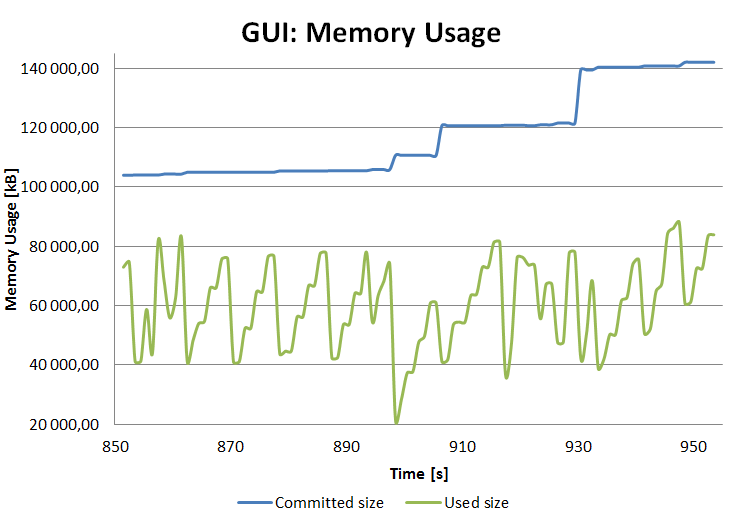
\includegraphics[width=0.6\textwidth]{prof_GUI_MEM}
  \caption{Profiling results of GUI component - memory usage perspective}
  \label{fig:prof_GUI_MEM}
\end{figure}

\subsection{Tests Results - Monitoring Hub module}

\begin{figure}[ht]
  \centering
  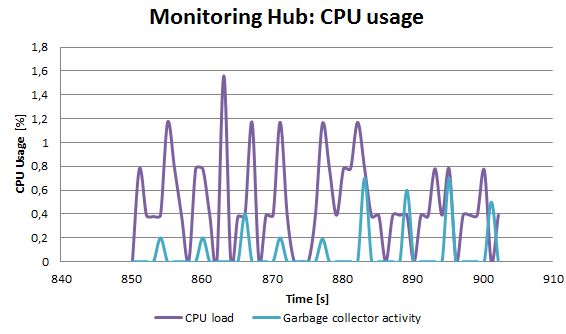
\includegraphics[width=0.6\textwidth]{prof_mon_hub_CPU}
  \caption{Profiling results of Monitoring Hub component - CPU usage perspective}
  \label{fig:prof_mon_hub_CPU}
\end{figure}


As can be easily predicted, Monitoring Hub module were consuming significantly smaller portion of resources then GUI. Figures~\ref{fig:prof_mon_hub_CPU}~and~\ref{fig:prof_mon_hub_mem} covers telemetry of Monitoring Hub JVM process in same time (step 9 of test scenario). As This module\rq{}s CPU usage was only fraction of GUI\rq{}s - peak was 1.6\% and all those results are near to measuring noise. Regarding memory usage - Those values also were smaller than in GUI but significant - memory actually used by application was staying in 10-20MB range, commit memory was nearly constant and equal to 50MB.

\begin{figure}[ht]
  \centering
  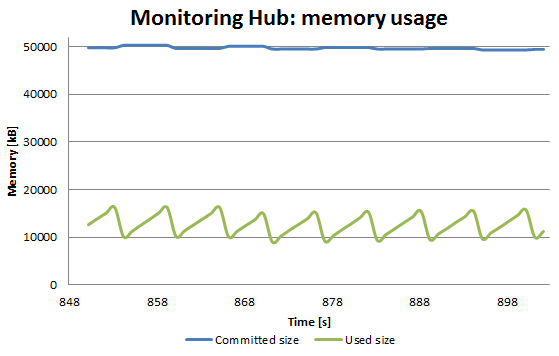
\includegraphics[width=0.6\textwidth]{prof_mon_hub_mem}
  \caption{Profiling results of Monitoring Hub component - memory usage perspective}
  \label{fig:prof_mon_hub_mem}
\end{figure}

\subsection{Tests Summary}

Test results showed clearly that performance of proposed system is good enough to. 
